\documentclass[11pt,a4paper]{article}
\usepackage[utf8]{inputenc}
\usepackage{amsmath}
\usepackage{amsfonts}
\usepackage{amssymb}
\usepackage{graphicx}
\usepackage{url}
\usepackage{enumitem}

\usepackage{listings}
\lstdefinelanguage{scala}{
  morekeywords={abstract,case,catch,class,def,%
    do,else,extends,false,final,finally,%
    for,if,implicit,import,match,mixin,%
    new,null,object,override,package,%
    private,protected,requires,return,sealed,%
    super,this,throw,trait,true,try,%
    type,val,var,while,with,yield},
  otherkeywords={=>,<-,<\%,<:,>:,\#,@},
  sensitive=true,
  morecomment=[l]{//},
  morecomment=[n]{/*}{*/},
  morestring=[b]",
  morestring=[b]',
  morestring=[b]"""
}

\usepackage{color}
\definecolor{dkgreen}{rgb}{0,0.6,0}
\definecolor{gray}{rgb}{0.5,0.5,0.5}
\definecolor{mauve}{rgb}{0.58,0,0.82}
\lstset{frame=tb,
  language=scala,
  aboveskip=3mm,
  belowskip=3mm,
  showstringspaces=false,
  columns=flexible,
  basicstyle={\small\ttfamily},
  numbers=none,
  numberstyle=\tiny\color{gray},
  keywordstyle=\color{blue},
  commentstyle=\color{dkgreen},
  stringstyle=\color{mauve},
  frame=single,
  breaklines=true,
  breakatwhitespace=true
  tabsize=3
}

\title{Semester project -- Pong Designer\\Theoretical report}
\author{\textit{Author:} Lomig Mégard\\
\textit{Supervisors:} Prof. Viktor Kuncak and Mikaël Mayer\vspace*{0.5cm}\\
\textsc{LARA/EPFL}}

\begin{document}
\maketitle

\section{Introduction}
This semester project came to support the Pong Designer project by Mikaël Mayer. The program was becoming increasingly large and suffered from a lack of global design. The home-made physics engine reached its limits in term of performance and precision. We decided to integrate a real physics engine together with some new clear design choices that would improve the future of the project. After some time, we concluded that it would be too complicated to take the current code and modify it. Therefore, I started almost from scratch the backbone of the new program. The majority of time was spent on design choices and the implementation of the basic bricks. There are the physics engine, the type system with its AST of expressions, the game objects that wrap physical ones and finally the system of rules. Each of these brick has been thought to be the more extensible and generic possible. The resulting project does not change the theoretical ideas behind Pong Designer, but refines its implementation and offers a stronger basis for further improvements.

In this report, I will begin with a description of Pong Designer and the principles it supports. Then, the type system behind the rules and expressions will be explained. The different rules and their properties will be listed. After that, I will talk more about the categories that are used to group objects with a common behaviour. I will also give more information to the chosen physics engine JBox2D. From a more technical point of view, the choice of fixed time step for the game engine will be explained. Finally, the possible future work and the conclusion will close this report.

\section{Programming by Demonstration}
The main idea of Pong Designer is to let the user define not only the state but also the behaviour of the game. Using a tablet, the user can program directly in the game and not through the code. This is achieved by the demonstration of the desired behaviour. The game engine takes care of inferring an appropriate rule to match the user wish. The user, who is now a developer, specifies the condition for the rule and modifies the current state to a final state. An example could be a collision that triggers a score increment. With these three information, the inferencer has to find a rule of the form: \textit{if there is a collision between these objects, then increment by one this score}. The set of rules is applied at each time step to modify the game state. A physics engine controls the physical behaviour of the objects. 

\section{Type system}
The central point of Pong designer is its rule system. It requires the ability to reason about them, to deconstruct a rule to modify only a subset of it. Indeed, we must offer to the user the possibility to change for example the value of a constant that lies deep into a rule statement. This need forbids the use of raw Scala to handle rule behaviour. The choice of an AST was simple since it is convenient to manipulate and modify in Scala. Each expression is thus evaluated by an interpreter at runtime. The following example shows a statement with its tree representation.
\begin{lstlisting}
circle("x") := circle("x") + 1
Assign(circle.x, Add(circle.x, IntegerLiteral(1)))
\end{lstlisting}

In order to be sure that an expression is correct, a system of dynamic type has been added to these trees. They are computed at runtime by the typechecker. For the moment, the following types are handled. They have a strong link to their corresponding Scala type. The translation in both directions is efficient and almost type safe.
\begin{itemize}[noitemsep,topsep=2pt,parsep=1pt,partopsep=1pt]
\item Integer
\item Float
\item String
\item Boolean
\item Pair of floats
\end{itemize}

\paragraph*{}
The game performances can suffer of the interpretation of rules. In a future, we could generate Scala code with the same behaviour as the trees. The compiled code would cohabits with its AST and thus benefits from both, in order to have the performance and the modularity.

\section{Rules}
In the Pong Designer game engine, the rules can change some properties value and thus the world state if their condition holds. They are immutable and use a boolean expression for their condition and a statement for the body. We wanted to have some rules to be executed only once per game run, without adding a boolean flag that would have complicated the code. Therefore, three types of rule are present:
\begin{itemize}[noitemsep,topsep=2pt,parsep=1pt,partopsep=1pt]
\item \texttt{Whenever}: triggered when the condition is satisfied
\item \texttt{On}: triggered when the condition change from false to true
\item \texttt{Once}: triggered only once when the condition is satisfied
\end{itemize}

\section{Categories of objects}
In the original Pong Designer, when a user duplicates an object all the rules associate with it are also copied. This leads to a large number of rules and a poor modularity. If we take the example of the Brick Breaker, a brick has to been build first with its rules and only after the user can duplicate it. Any behaviour modification wanted on all bricks require to modify them one by one the. To address this problem, we built a system of group, or category. With them, the user and the game engine can reason both at the level of a group of objects or at an atomic level. Each object has been assigned a category, and only one. In the future, we could remove this limitation to permit more sophisticated grouping but resulting in a more complex user interface. The following code snippet illustrates how to use categories. 

\begin{lstlisting}
val bricks = new Category("Bricks")
rectangle("b1", x = 1, y = 0).withCategory(bricks)
rectangle("b2", x = 3, y = 0).withCategory(bricks)

// ball and score definition not visible here
val rule = foreach(bricks) { brick =>
  whenever(Collision(ball, brick)) { Seq(
    brick("visible") := false, 
    score("value") += 1
  )}
}
\end{lstlisting}

We introduce the rule iterator \texttt{foreach} that takes care of generating, typecheking and evaluating the rules. The iteration can also occurs on multiples categories:

\begin{lstlisting}
val rule = foreach(cat1, cat2) { (o1, o2) => ... }
\end{lstlisting}

The process to obtain this elegant solution was long. The original one was accepting the categories directly in the rules. The problem that occurred rapidly was a lack of meaning in expressions. For example in the following code it was hard to know that the \texttt{brick} must be filled with the objects of the category \texttt{bricks}. In the general case with more than one category involved, the problem is even impossible to solve since not enough information is available to give the wanted behaviour to the rule.
\begin{lstlisting}
whenever(Collision(ball, bricks)) { brick => ... }
whenever(Collision(balls, bricks)) { (ball, brick) => ... }
\end{lstlisting}

\section{Physics engine}
The original goal if this project was to look at the physical engine used in the application and to find a way to improve it. That was especially needed since the implementation was suffering of tunnelling, namely when a physical object with a high velocity pass through another one. The physics engine was not the central point and it was a lost of time to maintain and debug. This is why we decided to integrate dedicated physics engine. 

I choose the project JBox2D\footnote{Website: \url{http://www.jbox2d.org/}} that exists for a long enough time to have good performances and a large community. For the moment we do not use all its features. Some could be useful in the future, for example the joins that permit to link two objects in multiple ways.

The architecture of JBox2D is based on the physical body. Each of them can have one or many shapes, defining its mass, center of mass, collision outline and other physical properties. To simplify the implementation, the principle of body has been kept in Pong Designer but some freedom have been removed. Particularly, each body has exactly one shape.

\section{Time management}
The time management is an important feature of Pong Designer. It permits to navigate through the past in order to select events and generate new rules. In the previous sections, we have seen multiple kinds of states: The objects properties, the rules, the asynchronous events. All these states must be part of the simulation history. At each time step end, the current state is stored only if different from the previous one. The game takes care of a discrete time counter for which the base unit is one \texttt{update} call. Each property or rule iterator is responsible of its own history. 

The history permits to \texttt{restore} the game to any past state given a specific discrete timestamp. Since the objects properties are separated from the physical simulation layer, we can replay the history efficiently and decide when flushing the new values to the physical layer and continue with a simulated environment. To limit the memory consumption, the history size is bounded by a constant. However, it is always possible to  \texttt{reset} the game to its initial state.

\section{Fixed time step}
During the integration of the physics engine, I had to choose between fixed time step variable time step. To understand the context, we need to look at one particular time step and decompose it. First, let FPS be the number of frames rendered per second and UPS be the number of times per second the word is updated, including the JBox2D step. Figure \ref{fig:variableTimeStep} shows the two phases \texttt{update} and \texttt{render}. 

\begin{figure*}[h]
\centering
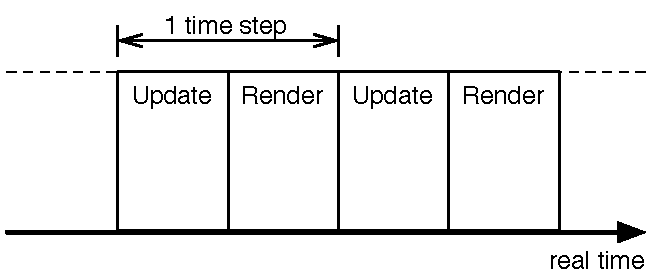
\includegraphics[scale = 0.8]{images/variableTimeStep} 
\caption{Variable time step.}
\label{fig:variableTimeStep}
\end{figure*}

With this simple approach, the FPS and UPS are variable. It is a problem because the physics simulation needs a fixed $\Delta t$ between two successive steps. At most, the difference should be little, which we cannot ensure with the previous design. Indeed, both the time to update the physical world and the one required to draw the objects on the screen are unpredictable due to the numerous factors that influence it. A thread can be preempt and thus slowed by the system, the number of objects do update and draw can change and, more specifically to our project, the number of rules to evaluate is variable. From the point of view of the user, the game could have different speeds on two devices and even during the simulation.

In order to have a fixed UPS, we introduce a sleeping period to synchronize all time steps as explained in \cite{FixYourTimestep, AndroidGameLoop}. Figure \ref{fig:fixedTimeStep} shows the result when we have effectively the time to sleep after both \texttt{update} and \texttt{render}. The thread that runs the game loop, updating and drawing the game, is depicted on the top part of the time line. The android thread which handle all events as user inputs is on the bottom. We observe that all asynchronous events are stored during an entire time step (including the sleep) and then shared with the game engine at the beginning of the next step.

\begin{figure*}[h]
\centering
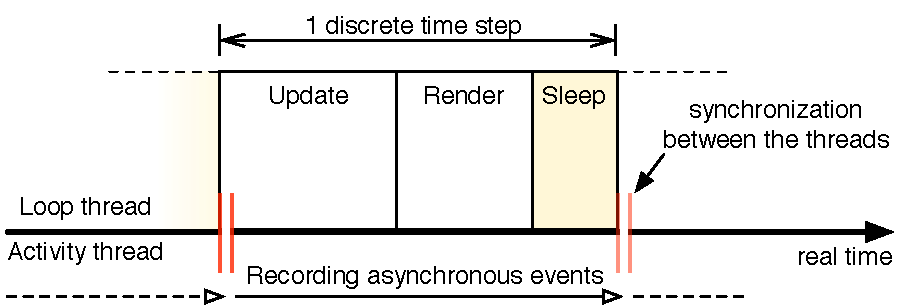
\includegraphics[scale = 0.8]{images/fixedTimeStep} 
\caption{Fixed time step.}
\label{fig:fixedTimeStep}
\end{figure*}

This technique ensure a constant UPS but not a constant FPS. Indeed, if the update and the rendering take more than the time allocated to one time step, we will perform two successive \texttt{update} to catch up. We see this case in figure \ref{fig:missFrame} where the first rendering is taking too much time. The second time step contains thus two updates, missing one frame, however the third time step can be performed normally. The result for the user is a constant and logical simulation with occasionally some missed frame. The visual feeling is better than with variable UPS.

\begin{figure*}[h]
\centering
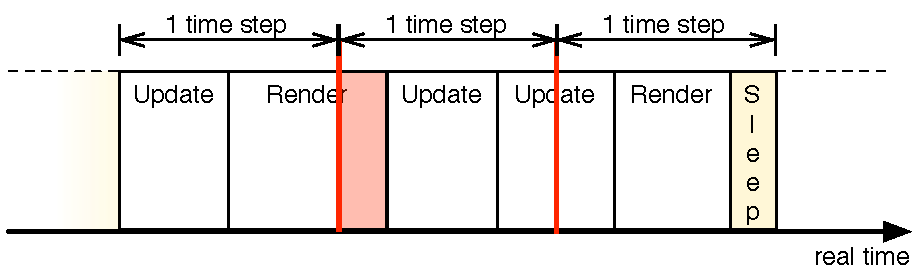
\includegraphics[scale = 0.8]{images/missFrame} 
\caption{Fixed time step with a missed frame.}
\label{fig:missFrame}
\end{figure*}

\clearpage
\section{Future work}
In this report, we go through some essential program bricks. The glue between them is a key process before programming the user interface and adding some logic. It has been partially coded, the API is ready to handle user inputs: new rules, time management, new objects and categories are all available. However, the rule inference, which is a major game engine logic, is still missing. The rule inference is the process to generate new rule from the difference between initial and final states. With the new ASTs of statements and expressions, the transfer of the old implementation to the new one should be fairly easy. It is clearly the domain where a lot of improvement is possible, as it touches to artificial intelligence and constraint solving. These are two areas where the solution is always a tradeoff between performance and precision and where the algorithms, if known, are often NP-Hard. I personally think that the inferencer is a key element in Pong Designer, perhaps with its user interface and the ability to go back in time.

The second step would be to implement the user interface. The API is given but all the graphical elements and the logic must be coded. Again, the old interface can be reused with only small modifications. The only new functionality to take care of is the categories management. In particular, the game engine has to decide whether a rule should apply to the specific object on which the demonstration has been done, or on its whole category.

\section{Conclusion}
This project began with pretentious goal: refactor a large program, improving particularly the physics engine. However, the integration of JBox2D gradually required other modification and we arrived at the point where almost all had to be recoded. The principles remained valid but the implementation needed a new design. I spent some time reading papers and talking with Mikaël Mayer to understand the context and the real problematic behind this project. The collaboration with Mikaël was interesting and rewarding. The different obstacles where a source of great discussions. They gave me the opportunity to better understand the issues that come with real projects. Particularly, the type system revealed the difficulty to deal with user inputs. 

At the end, there is still a lot of work to fulfil the original goals. Nevertheless, the objectives evolved during the semester and I am convinced that this project redefines all the main building blocks of the next version of Pong Designer. 


\clearpage
\nocite{*}
\bibliographystyle{plain}
\bibliography{bib}
\end{document}